\documentclass[12pt,a4paper]{article}
\usepackage[brazil]{babel}  %Suporte a PT-BR
%\usepackage[utf8]{inputenc} %Não necessário com XeLaTeX, suporta acentos
\usepackage{graphicx} %Importar imagens
\graphicspath{{./img/}}
\usepackage{amsmath} %Equações
\usepackage{float} %Inserir imagens in situ
\usepackage{listingsutf8} %Código com acentos
\usepackage[backend=biber]{biblatex} %Suporte à Bibliografia
\addbibresource{references.bib}

\title{Relatório da Atividade de Escalonamento}
\author{Vítor Barbosa}
\date{\today}

\begin{document}
\maketitle

\section*{Introdução}
Vamos verificar se as tarefas na tabela \ref{table:1} são escalonáveis.

\begin{table}[H]
\centering
\begin{tabular}{|c|c|c|c|c|}
\hline
Tarefas &
  \begin{tabular}[c]{@{}c@{}}Jitter\\ $(J_i)$\end{tabular} &
  \begin{tabular}[c]{@{}c@{}}Computing\\ Time $(C_i)$\end{tabular} &
  \begin{tabular}[c]{@{}c@{}}Período \\ $(P_i)$\end{tabular} &
  \begin{tabular}[c]{@{}c@{}}Deadline\\ $(D_i)$\end{tabular} \\ \hline
Tarefa 1 & 10 & 10 & 40 & 40 \\ \hline
Tarefa 2 & 5  & 10 & 80 & 25 \\ \hline
Tarefa 3 &    & 5  & 80 & 40 \\ \hline
Tarefa 4 &    & 10 & 40 & 40 \\ \hline
Tarefa 5 & 10 & 5  & 80 & 40 \\ \hline
Tarefa 6 &    & 10 & 40 & 80 \\ \hline
\end{tabular}
\caption{Conjunto de Tarefas para análise}
\label{table:1}
\end{table}

As equações que serão usadas são:
 
\begin{itemize}
\item  A n-ésima Janela da Tarefa i:
\begin{equation}
W_i^n=C_i+ \sum_{j \in hp(i)} \left\lceil\frac{W_i^{n-1}+J_j}{P_j}\right\rceil C_j 
\end{equation}
\item O tempo de resposta da Tarefa i:
\begin{equation}
R_i=W_i+J_i
\end{equation}
\item A utilização do processador
\begin{equation}
U_i=\frac{C_i}{P_i}
\end{equation}
\end{itemize}

Uma tarefa é dada como escalonável se :
\begin{equation}
R_i\leq D_i
\end{equation}

O conjunto de tarefas é dado como escalonável se:
\begin{equation}
U=\sum U_i \leq m
\end{equation}
Sendo m o número de processadores.

\section*{1-Grafo do Sistema}
O grafo proposto para todas as tarefas do sistema está na figura \ref{grafo}.

\begin{figure}[H]
\centering
\includegraphics[width=0.5\textwidth]{grafo_tarefas}
\caption{Grafo com Todas as Tarefas}
\label{grafo}
\end{figure}

\section*{2-Verificar se cada tarefa é escalonável}
\subsubsection*{Tarefa 1 (T1)}
\begin{gather*}
W_1^0 = C_1 = 10\\
R_1=W_1+J_1 = 10+10=20 \leq 40
\end{gather*}
A tarefa 1 é escalonável.
\subsubsection*{Tarefa 2 (T2)}
A tarefa 2 sofre interferência da tarefa 1, que é mais prioritária.
\begin{gather*}
W_2^0 = C_2 = 10 \\
W_2^1= C_2 + \left\lceil\frac{W_2^0+J_1}{P_1}\right\rceil C_1 = 10 + \left\lceil\frac{10+10}{40}\right\rceil  10 = 20 \\
W_2^2=C_2+\left\lceil\frac{W_2^1+J_1}{P_1}\right\rceil  C_1 = 10+\left\lceil\frac{20+10}{40}\right\rceil  10 = 20\\
R_2=W_2+J_2=20+5=25\leq 25
\end{gather*}
A tarefa 2 é escalonável, ficando no limite de seu deadline.

\subsubsection*{Tarefa 3 (T3)}
A T3 sofre interferência da T1 (mais prioritária) e um jitter extra igual ao tempo de resposta de T2 porque depende da conclusão de T2.
\begin{gather*}
W_3^0 = C_3 = 5 \\
W_3^1= C_3 + \left\lceil\frac{W_3^0+J_1}{P_1}\right\rceil C_1 = 5 + \left\lceil\frac{5+10}{40}\right\rceil  10 = 15 \\
W_3^2= 5 + \left\lceil\frac{15+10}{40}\right\rceil  10 = 15\\
R_3=W_3+J_3+R_2=15+0+25=40\leq 40
\end{gather*}
A tarefa 3 é escalonável, ficando no limite de seu deadline.

\subsubsection*{Tarefa 4 (T4)}
\begin{gather*}
W_4^0 = C_4 = 10 \\
W_4^1= C_4 + \left\lceil\frac{W_4^0+J_1}{P_1}\right\rceil C_1 + \left\lceil\frac{W_4^0+J_2}{P_2}\right\rceil C_2 + \left\lceil\frac{W_4^0+J_3}{P_3}\right\rceil C_3 \\
W_4^1= 10 + \left\lceil\frac{10+10}{40}\right\rceil 10 + \left\lceil\frac{10+5}{80}\right\rceil 10 + \left\lceil\frac{10+25}{80}\right\rceil 5 =35\\
\end{gather*}
É evidente que $W_4^2 > D_4$ e portanto a T4 não é escalonável em um processador só. 

Como temos 3 processadores, vamos dividir as tarefas assim:

\begin{itemize}
\item Processador 1 $\rightarrow$ Tarefas T1, T2 e T3
\item Processador 2 $\rightarrow$ Tarefa T4
\item Processador 3 $\rightarrow$ Tarefas T5 e T6
\end{itemize}
Deste modo, a T4 roda sozinha no processador 2 e não sofre interferência das outras tarefas e temos:
\begin{gather*}
W_4^0 = C_4 = 10 \\
R_4=W_4+J_4 = 10+0=10 \leq 40
\end{gather*}
Agora, a T4 é escalonável.
\subsubsection*{Tarefa 5 (T5)}
A T5 é a tarefa mais prioritária do processador 3.
\begin{gather*}
W_5^0 = C_5 = 5 \\
R_5=W_5+J_5 = 5+10=15 \leq 40
\end{gather*}
A T5 é escalonável.
\medskip

\subsubsection*{Tarefa 6 (T6)}
A T6 é possui Deadline maior que o Período e portanto não pode entrar na análise de escalonabilidade que estamos aplicando.

\section*{3-Calcular os Tempos de Resposta Máximos}
Os tempos de resposta já foram calculados no item anterior, eles estão dispostos na tabela \ref{table:2}.
\begin{table}[H]
\centering
\begin{tabular}{|c|c|}
\hline
\multicolumn{1}{|l|}{Tarefa} & \multicolumn{1}{l|}{Tempo de Resposta} \\ \hline
Tarefa 1                     & 20                                     \\ \hline
Tarefa 2                     & 25                                     \\ \hline
Tarefa 3                     & 40                                     \\ \hline
Tarefa 4                     & 10                                     \\ \hline
Tarefa 5                     & 15                                     \\ \hline
Tarefa 6                     &                                        \\ \hline
\end{tabular}
\caption{Tempos de Resposta das tarefas}
\label{table:2}
\end{table}

\section*{4-Verificar a Utilização do Processador}
\begin{gather*}
U=\sum U_i = \sum\frac{C_i}{P_i}\\
U = \frac{C_1}{P_1} +  \frac{C_2}{P_2} +  \frac{C_3}{P_3} +  \frac{C_4}{P_4} +  \frac{C_5}{P_5}\\
U =  \frac{10}{40} +  \frac{10}{80} +  \frac{5}{80} +  \frac{10}{40} +  \frac{5}{80} = 0.75
\end{gather*}
A utilização (excluída a tarefa 6) é de 0.75. Como ela é menor que o número de processadores (3), o conjunto de tarefas é escalonável.
\printbibliography

\end{document}